\fancyhead[RO,LE]{\thepage}
\fancyfoot{} 
\chapter{Evaluation}
\label{chapter:evaluation}

In the previous chapter I presented a massively parallel GPU algorithm for level set segmentation. In this chapter I describe a methodology for evaluating this algorithm. I analyze the asymptotic performance and memory efficiency of my algorithm. I also describe a series of experiments that compare the computational efficiency and accuracy of my GPU algorithm to the previous state-of-the-art GPU algorithm.
The results of these experiments show that my algorithm significantly outperforms previous state-of-the-art algorithms with no reduction in segmentation accuracy.%-------------------------------------------------------------------------
\section{Asymptotic Complexity}
\label{subsec:asymptoticComplexity}

The algorithm I use for buffer compacting has $O(w)$ work-complexity and $O({\log }_{2}w)$ step-complexity where $w$ is the size of the input~\cite{Sengupta-2011}. Therefore my algorithm has $O(p)$ work-complexity and $ O \leftbracket { \log }_2 p \rightbracket $ step-complexity during initialization where $p$ is the size of the entire level set field. After initialization my algorithm has $O(n)$ work-complexity and $ O \leftbracket { \log }_2 n \rightbracket $ step-complexity where $n$ is the size of the active computational domain. From this I conclude that my algorithm is both work-efficient and step-efficient. For a more detailed proof I refer the reader to Appendix~\ref{app:proof}.

My algorithm requires $O(p)$ memory. In other words the memory requirements of my algorithm increase linearly with the size of the level set field rather than the (much smaller) surface area of the segmented surface, as is the case with previous GPU algorithms~\cite{Lefohn-2003-MICCAI,Lefohn-2003-Vis,Cates-2004,Lefohn-2004,Jeong-2009}.

%-------------------------------------------------------------------------
\section{Experimental Methodology}
\label{subsec:experimentalMethodology}


I performed all my experiments on an Intel 2.5 gigahertz Xeon Processor with 4 gigabytes of memory and an NVIDIA GTX 280 GPU. I implemented my algorithm using CUDA~\cite{NVIDIACUDA-2010} and I used the open-source CUDA Data Parallel Primitives Library~\cite{CUDPP-2010} for buffer compacting. I implemented the GPU narrow band algorithm using OpenGL~\cite{Shreiner-2005} and GLSL~\cite{Rost-2006} with a tile size of $16^2$, as described by Lefohn et al.~\cite{Lefohn-2003-MICCAI,Lefohn-2003-Vis,Lefohn-2004}. I feel this is the fairest method of evaluating each algorithm since the GPU narrow band algorithm relies on hardware features not exposed in CUDA (e.g. direct write access to texture memory). Likewise my algorithm makes use of hardware features not exposed in OpenGL and GLSL (e.g. random write access to global memory).

I performed various segmentation tasks on volumetric images generated from the BrainWeb Simulated Brain Database~\cite{BrainWeb-2010,Kwan-1996,Cocosco-1997,Collins-1998,Kwan-1999}. This database can be used to generate simulated head MRIs with a variety of realistic noise characteristics in a controlled setting where the ground truth classification of each voxel is known. I repeated these segmentation tasks using my algorithm, the GPU narrow band algorithm, and a level set solver implemented in CUDA that unconditionally updates the entire level set field. I also performed various segmentation tasks on a $256 \times 256 \times 272$ abdominal CT image and a $288 \times 352 \times 112$ wrist CT image using my algorithm.

To evaluate the accuracy and variability of my algorithm, I performed a series of repeated ($N=10$) white matter segmentations on ${256}^3$ head MRIs with varying signal-to-noise ratio (SNR) values. I segmented these images using a randomly selected seed location. I measured the accuracy of each segmentation by computing the Dice Coefficient~\cite{Shattuck-2009,Jeong-2009} and the Total Correct Fraction~\cite{Lefohn-2003-MICCAI,Cates-2004}.

To evaluate the speed of my algorithm, I segmented the white and grey matter in a ${256}^3$ head MRI with $SNR=11$. I measured the computation time per iteration per subroutine and the total computation time for the segmentation. I also measured the number of active voxels per iteration and the total number of processed voxels. To provide additional context for these experiments, I repeated the segmentation task using the open-source Insight Segmentation and Registration Toolkit~\cite{Ibanez-2005}, which implements the sparse field algorithm~\cite{Whitaker-1998,Peng-1999} in single-threaded C++.

\section{Results and Discussion}

%*******************************************************************************
% FIGURE Aorta
\begin{figure}[t]
\centering
\includegraphics[width=6.0in]{figures/Aorta-3D.png}
\caption{The aorta and kidneys in a $256 \times 256 \times 272$ abdominal CT image segmented with my algorithm. The total computation time required to produce this segmentation was 16 seconds.}
\label{fig:aorta}
\end{figure}
%*******************************************************************************

%*******************************************************************************
% FIGURE Bone
\begin{figure}[t]
\centering
\includegraphics[width=6.0in]{figures/Bone-3D.png}
\caption{The cortical bone and trabecular bone in a $288 \times 352 \times 112$ wrist CT image segmented with my algorithm. The total computation time required to produce this segmentation was 12 seconds.}
\label{fig:bone}
\end{figure}
%*******************************************************************************

%*******************************************************************************
% FIGURE BrainWeb 3D
\begin{figure}[t]
\centering
\includegraphics[width=6.0in]{figures/Brainweb-3D-Composite-NoText.png}
\caption{The progression of my algorithm while segmenting the white and grey matter in a $256^3$ head MRI with a signal-to-noise ratio of 11. The total computation time required to produce this segmentation was 7 seconds.}
\label{fig:brainweb3d}
\end{figure}
%*******************************************************************************

%*******************************************************************************
% FIGURE BrainWeb 2D
\begin{figure}[t]
\centering
\includegraphics[width=6.0in]{figures/Brainweb-2D-Composite-2-3.png}
\caption{The progression of the active computational domain (shown in blue) with my algorithm while segmenting the white matter in a $256^3$ head MRI. Regions that have locally converged are immediately marked as inactive due to my analysis of the temporal and spatial derivatives of the level set field. The size of the active computational domain drops to zero when the segmentation has globally converged.}
\label{fig:brainweb2d}
\end{figure}
%*******************************************************************************
%*******************************************************************************
% FIGURE Accuracy
\begin{figure}[t]
\centering
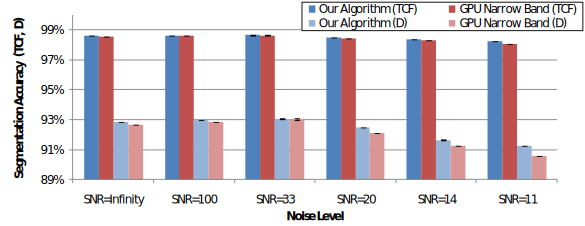
\includegraphics[width=6.0in]{figures/Accuracy.pdf}
\caption{Accuracy of my algorithm and the GPU narrow band algorithm while performing a set of repeated (N=10) white matter segmentations in a $256^3$ head MRI with varying signal-to-noise-ratio (SNR) values. For each segmentation I used a randomly selected seed point and I measured the Dice Coefficient (D) and Total Correct Fraction (TCF).}
\label{fig:8}
\end{figure}
%*******************************************************************************

%*******************************************************************************
% FIGURE Active Computational Domain per Iteration
\begin{figure}[t]
\centering
\includegraphics[width=6.0in]{figures/SpeedA1.pdf}
\caption{Size of the active computational domain per iteration for my algorithm and the GPU narrow band algorithm while segmenting the white and grey matter in a $256^3$ head MRI. The total number of grid elements processed by each algorithm is the definite integral of that algorithm's curve on this plot. These integrals are shown in the inset. Lower is better.}
\label{fig:activecomp}
\end{figure}
%*******************************************************************************

%*******************************************************************************
% FIGURE Speed per Iteration
\begin{figure}[t]
\centering
\includegraphics[width=6.0in]{figures/SpeedB1.pdf}
\caption{Computation time per iteration for my algorithm and the GPU narrow band algorithm while segmenting the white and grey matter in a $256^3$ head MRI. The total computation time for each algorithm is the integral of that algorithm's curve on this plot. These integrals are shown in the inset. Lower is better.}
\label{fig:speed}
\end{figure}
%*******************************************************************************

%*******************************************************************************
% FIGURE Speed per Active Computational Domain
\begin{figure}[t]
\centering
\includegraphics[width=6.0in]{figures/SpeedC1.pdf}
\caption{Computation time as a function of active computational domain size for my algorithm and the GPU narrow band algorithm while segmenting the white and grey matter in a $256^3$ head MRI. I overlay the lines of best fit for each algorithm. Lower is better.}
\label{fig:speedperactive}
\end{figure}
%*******************************************************************************

%*******************************************************************************
% FIGURE Speed per Subroutine
\begin{figure}[t]
\centering
\includegraphics[width=6.0in]{figures/SpeedD1.pdf}
\caption{Computation time per iteration for each subroutine of my algorithm while segmenting the white and grey matter in a $256^3$ head MRI. Lower is better.}
\label{fig:speedpersubroutine}
\end{figure}
%*******************************************************************************

Figure~\ref{fig:aorta} and Figure~\ref{fig:bone} show qualitatively accurate segmentations produced with my algorithm. Figure~\ref{fig:brainweb3d} shows the progression of my algorithm while segmenting the white and grey matter in a ${256}^3$ head MRI with $SNR=11$. Figure~\ref{fig:brainweb2d} shows the progression of the active computational domain while segmenting the white matter in the same MRI.

I compare the accuracy of my algorithm and the GPU narrow band algorithm in Figure~\ref{fig:8}. I observed that my algorithm was slightly more accurate than the GPU narrow band algorithm with less than 0.2\% variability in all experiments. I speculate that this slight accuracy improvement is due to different floating point precision semantics in CUDA and GLSL. The accuracies I observed are comparable to those reported by Lefohn et al.~\cite{Lefohn-2003-MICCAI} and Cates et al.~\cite{Cates-2004}.

I compare the performance of my algorithm and the GPU narrow band algorithm in Figure~\ref{fig:activecomp} and Figure~\ref{fig:speed}. I observed that with my algorithm, the number of active voxels quickly peaked and decreased over time due to my analysis of the temporal and spatial derivatives of the level set field. With the GPU narrow band algorithm, the number of active voxels monotonically increased over time (Figure~\ref{fig:activecomp}). I observed that after the number of active voxels had peaked, the speed of my algorithm increased over time in contrast to the GPU narrow band algorithm (Figure~\ref{fig:speed}).

I observed that segmenting the white and grey matter in a ${256}^3$ T1w MRI with $SNR=11$ using the Insight Segmentation and Registration Toolkit took 81 minutes and 4 seconds.

Based on the observed linear relationships between the number of active voxels per iteration and the computation time per iteration (Figure~\ref{fig:speedperactive}), I conclude that the computational domain would need to be roughly 12\% active before unconditionally updating every voxel would provide a performance benefit over my algorithm. At first glance it may seem as though the GPU narrow band algorithm would provide a performance benefit over my algorithm after the computational domain is roughly 9\% active. However due to the GPU narrow band algorithm processing data in 2D tiles of size $g^2$, an active computational domain of size $n$ using my algorithm will result in a larger active computational domain of size $q$ where $n\le q\le g^2n$ using the GPU narrow band algorithm. I observed that the computational domain remained less than 2\% active during each iteration of my algorithm in all experiments.


I observed that tracking the active computational domain using my algorithm accounted for 77\% of the total computation time and updating the level set field accounted for the remaining 23\% of the total computation time (Figure~\ref{fig:speedpersubroutine}). I conclude that although most of my computation time goes into tracking the active computational domain, I leverage this cost to avoid the bigger downstream cost of unconditionally updating the entire level set field.

